\section{Auswirkungen von unterschiedlichen Kameraauflösungen}
\label{sec:minimalAuf} 

Der entstandene Szenenrekonstruktionsalforithmus wurde anhand von Kameras gleicher Auflösung implementiert und bereits validiert. Im folgenden soll nun getestet werden, ob der entwickelte Algorithmus auch im Stande ist für Kameras unterschiedlicher Auflösung eine Szene richtig zu Rekonstruieren. Zunächst wird beschrieben, welche Modifizierungen auf einem Sensor bei veränderung Der Auflösung stattfinden. Anschließend wird analysiert, wie sich die Auflösungsänderung auf das in Kapitel \ref{sec:CameraModels} beschriebene Kameramodell ändert und welche Einflüsse sie auf die in Kapitel \ref{sec:HFE} hergeleiteten Epipolaren Bedingungen und somit auf die Bestimmung der extrinsischen Kameraparameter und der folgenden Szenenrekonstruktion hat. Zum Schluss werden die Ergebnisse der synthetischen Rekonstruktion mit unterschiedlichen Kameraauflösungen präsentiert und validiert.
 

\section{Geometrie eines Sensors}


Die Geometrie eines Sensors kann als eine  $M \times N$ - Matrix, bestehend aus $M \times N$ Sensorelementen dargestellt werden\cite{Photonik}. Die Auflösung eines Sensors hängt von den horizontalen und vertikalen Abständen der Sensorelemente ab. Abbildung \ref{fig:Sensor} zeigt den schematischen Aufbau eines Sensors (CMOS). \\


Ein Sensor hat eine maximale Auflösung. Die maximale Anzahl der Sensorelemente auf einem Sensor beschreit die maximale Auflösung. Verschiedene Kameras können aus diesem Grund verschiedenen Auflösungen besitzen. Die Anzahl und Größe der Einzelnen Sensorelemente variiert mit den Größen der Sensorchips. Je größer ein Sensor ist und je mehr Sensorelemente er besitzt, desto besser ist die Bildqualität\cite{Photonik}. Bei maximaler Auflösung definiert genau ein Sensorelement einen Pixel. Ein Pixel wiederum entspricht einem Bildpunkt\cite{Photonik}. Auch ist es möglich die Auflösung eines Sensors digital zu verändern. Wird eine Auflöung kleiner der maximalen Auflösung eingesteltt, desto geringer wird die Anzahl der Pixel. Der Prozess, welcher hier stattfindet, gehört zu den Nachbarschaftsoperationen. Benachbarte Pixel werden hier zu einem neuen Pixel definiert\cite{Photonik}. Ein neuer Pixel wird aus den benachbarten Pixeln berechnet.\\

\begin{figure}[!htb]
	\centering
	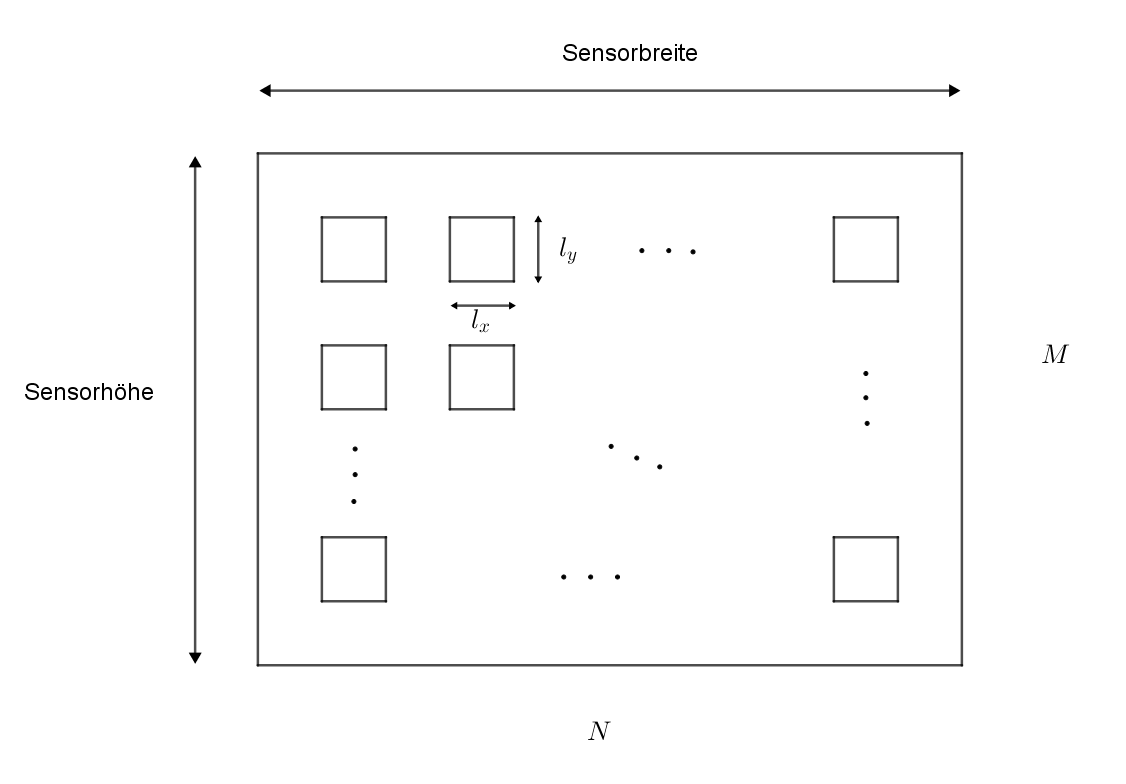
\includegraphics[width=.8\linewidth]{images/Bildsensor_mit_Pixel.png}
	\caption[Aufbau CMOS Sensor]{Rechteckiger Bildsensor mit darauf sich befindendenden quadratischen Sensorelementen. Vergleiche \cite{Photonik}} 
	\label{fig:Sensor}
\end{figure}
\pagebreak

Eine Veränderung der Auflösung kann auch eine Änderung der Seitenverhältnisse mit einschließen. Ändert sich das Seitenverhältnis so wird der Bereich der lichtempfindlichen Fläche auf dem Sensor beschränkt\cite{Photonik}. Dies führt dazu, dass sich die Bildausschnnitte ändern. Abbildung \ref{fig:SensorResolutions} stellt schematisch da wie sich die lichtempfindlichen Bereiche auf dem Sensor bei unterschiedlichen Auflösungen ändert.

%\pagebreak





%\begin{minipage}{\linewidth}
%	\centering
%	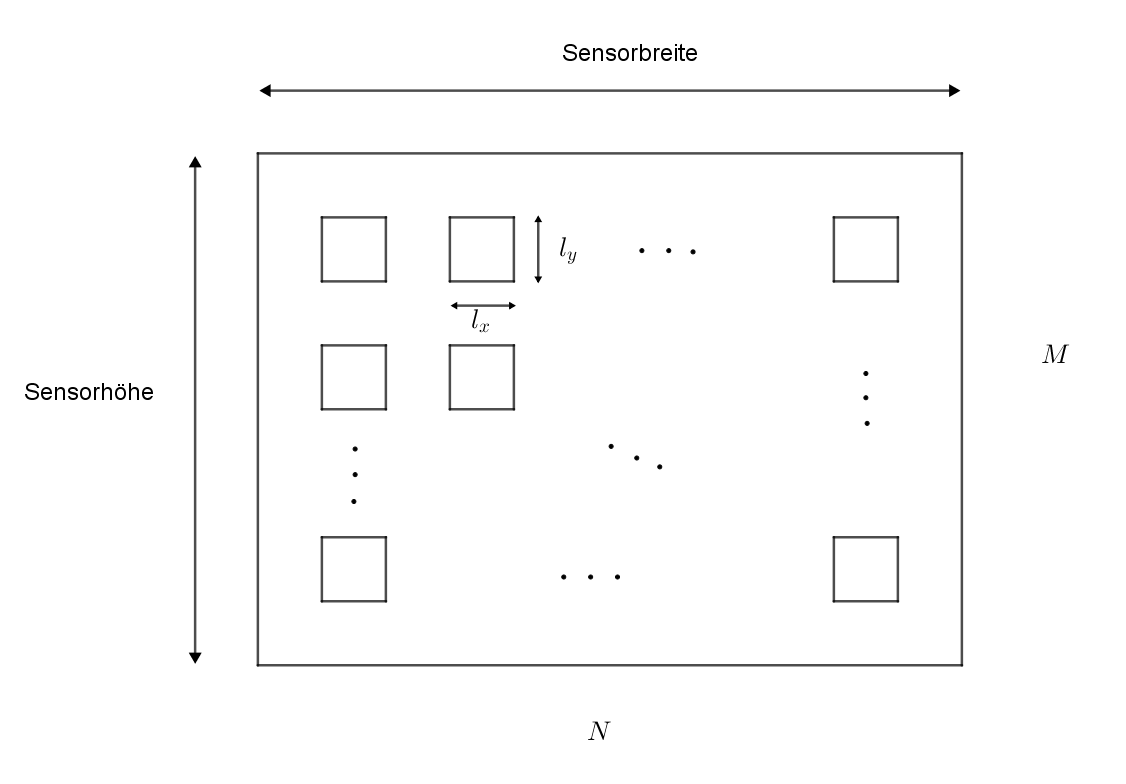
\includegraphics[width=.8\linewidth]{images/Bildsensor_mit_Pixel.png}
%	\captionof{figure}{Rechteckiger Bildsensor mit darauf sich befindendenden quadratischen Sensorelementen. Vergleiche \cite{Photonik}} 
%	\label{fig:Sensor}
%\end{minipage}\\\\

%
%Ein Sensor hat eine maximale Auflösung. Die maximale Anzahl der Sensorelemente auf einem Sensor beschreit die maximale Auflösung. Verschiedene Kameras können aus diesem Grund verschiedenen Auflösungen besitzen. Die Anzahl und Größe der Einzelnen Sensorelemente variiert mit den Größen der Sensorchips. Je größer ein Sensor ist und je mehr Sensorelemente er besitzt, desto besser ist die Bildqualität\cite{Photonik}. Bei maximaler Auflösung definiert genau ein Sensorelement einen Pixel. Ein Pixel wiederum entspricht einem Bildpunkt\cite{Photonik}. Auch ist es möglich die Auflösung eines Sensors digital zu verändern. Wird eine Auflöung kleiner der maximalen Auflösung eingesteltt, desto geringer wird die Anzahl der Pixel. Der Prozess, welcher hier stattfindet, gehört zu den Nachbarschaftsoperationen. Benachbarte Pixel werden hier zu einem neuen Pixel definiert\cite{Photonik}. Ein neuer Pixel wird aus den benachbarten Pixeln berechnet.\\
\begin{figure}[!htb]
	\centering
	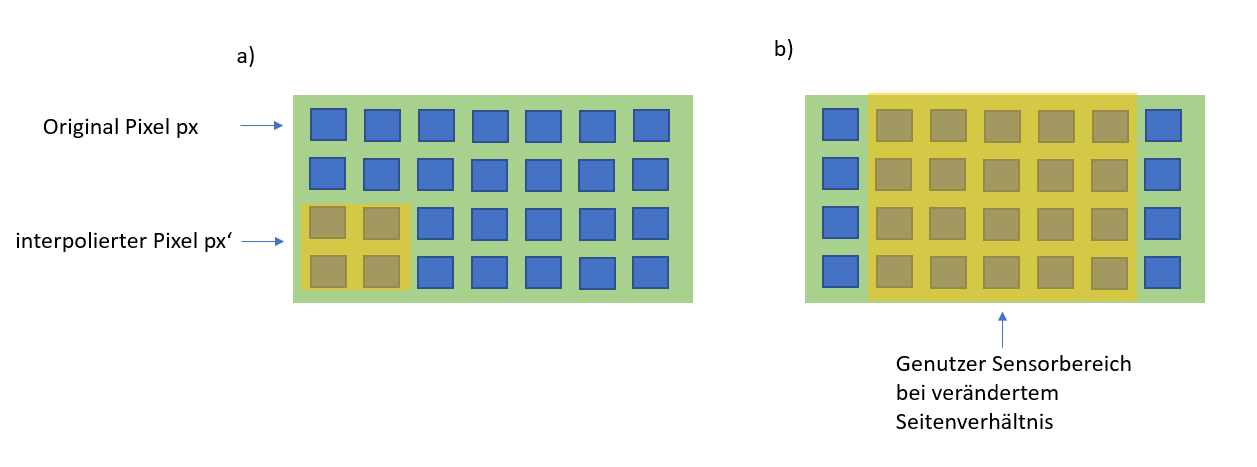
\includegraphics[width=1.\linewidth]{images/AufloesungSensor.png}
	\caption[Nachbarschaftsoperation auf Sensoren]{Bild a) zeigt die den Zusammenschluss mehrerer benachbarter Pixel zu einem neuen Pixel. Bild b) zeigt in gelb markiert, den aktiven lichtempfindlichen Bereich des Sensors, wenn sich das Seitenverhältnis geändert wird und nicht mehr der komplette Sensor genutzt wird.} 
	\label{fig:SensorResolutions}
\end{figure}


%
%Eine Veränderung der Auflösung kann auch eine Änderung der Seitenverhältnisse mit einschließen. Ändert sich das Seitenverhältnis so wird der Bereich der lichtempfindlichen Fläche auf dem Sensor beschränkt\cite{Photonik}. Dies führt dazu, dass sich die Bildausschnnitte ändern. Abbildung \ref{fig:SensorResolutions} stellt schematisch da wie sich die lichtempfindlichen Bereiche auf dem Sensor bei unterschiedlichen Auflösungen ändert.





\pagebreak

\section{Auswirkungen auf die Szenenrekonstruktion}

Im folgenden wird zunächst analysiert, welche Änderungen sich im Lochkameramodell bei veränderter Auflösung ergeben und was für Auswirkungen diese auf die in Kapitel \ref{sec:HFE} aufgestellten Epipolaren Bedingungen hat.\\

Im Lochkameramodell hat eine Änderung der Kameraauflösung lediglich eine Auswirkung auf die Skalierung der Sensorkoordinatenachsen. Mit der Auflösung, ändern sich die Anzahl und die Größe der Pixel. Die Längeneinheiten des Sensorkoordinatensystems orientieren sich, wie in Kapitel \ref{sec:CameraModels} beschrieben, an genau diesen Längenskalierung der Pixelkanten $l_x$ und $l_y$. Folglich kommt es zu einer Skalierung des Sensorkoordinatensystems.Alle anderen Koordinatensysteme bleiben unverändert. Durch Nachbarschaftsopterationen werden aus mehreren benachbarten Pixel ein neuer, jedoch bleibt der Ort des Pixel der gleiche\cite{Doessel}. Die Abbildungen \ref{fig:Aufl1} und \ref{fig:Aufl2} zeigen, dass sich zwar die Projektion von Bildebenenkoordinatensystem auf das Sensorkoordinatensystem für den Punkt $m_\sigma$ ändert, 

%Jedoch wird der Bildpunkt $m_{\tau'}$ an der selben Position des Sensors wie zuvor auch abgebildet.\\


%Eine Änderung der Kameraauflösung hat im Lochkameramodell lediglich eine Auswirkung auf die skalierung der Längeneinheiten des Sensorkoordinatensystems.

 
%Daraus wird geschlossen, dass sich die Koordinaten eines Punktes $m_\sigma$ mit den Pixelgrößen skaliert, jedoch bleiben seine Koordinaten bezüglich aller anderen Koordinatensysteme gleich.

%Während sich für dein Punkt im Sensorkoordinatensystem neue skalierte Koordinaten ergeben, so bleibt der Bildpunkt in Bildebenenkoordinaten unverändert. 



\begin{figure}[!htb]
	\minipage{0.48\textwidth}
	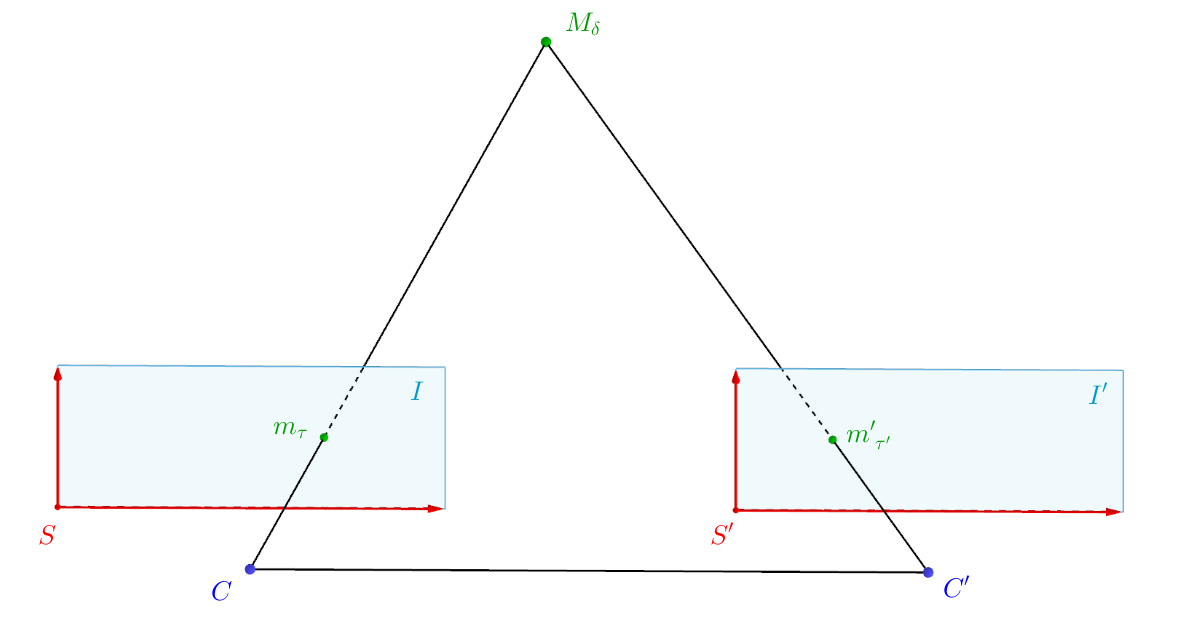
\includegraphics[width=\linewidth]{images/SensorSelbeAufloesung_beschriftet.png}
	\caption[Sensorkoordinatensystem bei Kameras gleicher Auflösung]{$C$ und $C'$ haben die selbe Auflösung eingestellt}
	\label{fig:Aufl1}
	\endminipage\hfill
	\minipage{0.49\textwidth}
	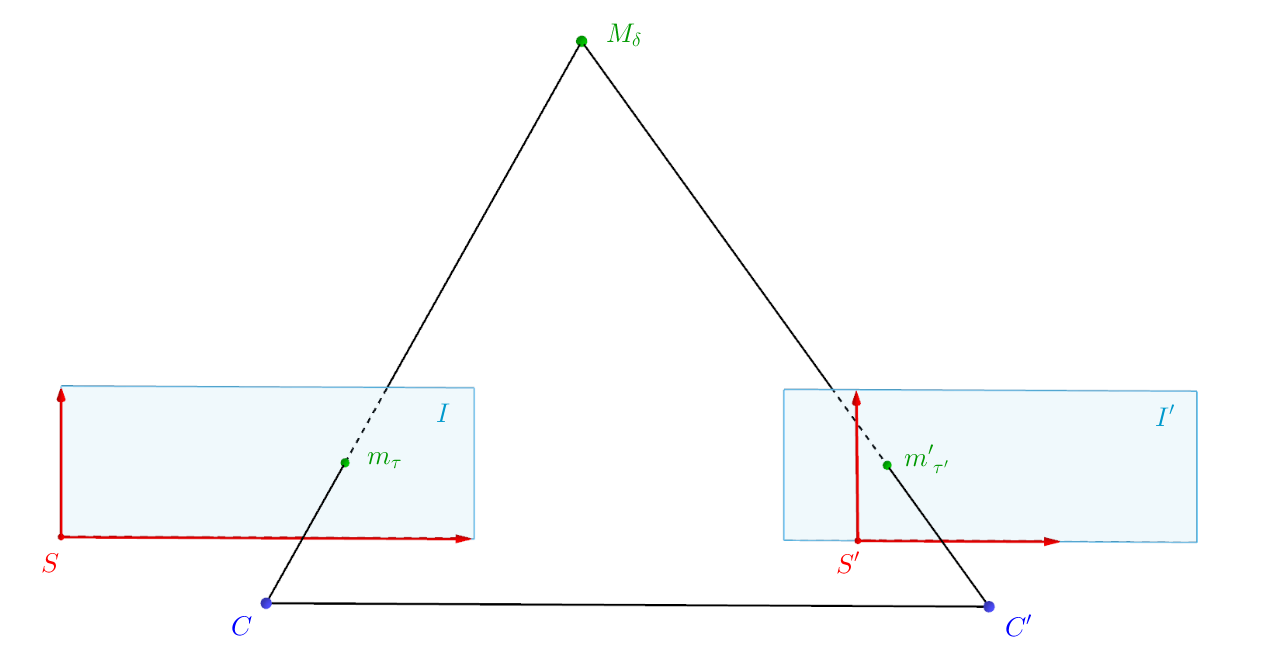
\includegraphics[width=\linewidth]{images/SensorUnterschiedlicheAufloesung_beschriftet.png}
	\caption[Sensorkoordinatensystem bei Kameras unterschiedlicher Auflösung]{$C$ und $C'$ haben unterschiedliche Auflösungen eingestellt}
	\label{fig:Aufl2}
	\endminipage\hfill
\end{figure}


Eine Skalierung der Sensorkoordinaten bedeutet, dass sich die Brennweite in Pixeleinheiten gegeben ändert, jedoch ändert sich nicht die effektive Brennweite in Millimeter. Anhand des Aufbau der Kameramatrix aus Kapitel \ref{sec:CameraModels} kann das nochmal verdeutlicht werden. 
%gezeigt, setzt sich die erweiterte Kameramatrix $K$ wie folgt zusammen:

\begin{equation}
K=  \begin{bmatrix}
k_x \zeta & 0 & V_{\sigma x}\\
0 & k_y \zeta & V_{\sigma y}\\
0 & 0   & 1 \\
\end{bmatrix}
\end{equation}

Wie bereits bekannt wird kommt es bei der Transformation von Bildebenenkoordinaten $m_\tau$ auf Sensorkoordinaten $m_\sigma$ zu einer Skalierung der Bildebenenkoordinaten in Millimeter auf Sensorkoordinaten in Pixel. $\zeta_x$ und $\zeta_y$ stehen für die Brennweite. Durch die Multiplikation mit $k_x$ und $k_y$ wird die Brennweite auf Pixeleinheiten skaliert. Die ursprüngliche Brennweite beträgt $\zeta_x = \zeta_y = 1$. Kommt jetzt eine skalierung von $k_x = k_y = 2$ dazu. 


\begin{gather}
	K_0=  \begin{bmatrix}
		\zeta & 0 & V_{\tau x}\\
		0 & \zeta & V_{\tau y}\\
		0 & 0   & 1 
	\end{bmatrix} =
	\begin{bmatrix}
	1 & 0 &  V_{\tau x}\\
	0 & 1 &  V_{\tau y}\\
	0 & 0 & 1 
\end{bmatrix}\\
	K= \begin{bmatrix}
		k_x \zeta & 0 & k_x V_{\tau x}\\
		0 & k_y \zeta & k_y V_{\tau y}\\
		0 & 0   & 1 
	\end{bmatrix} =
	\begin{bmatrix}
	2 \cdot 1 & 0 & 2 \cdot V_{\tau x}\\
	0 & 2 \cdot 1 & 2 \cdot V_{\tau y}\\
	0 & 0   & 1 
\end{bmatrix} = 
\begin{bmatrix}
	2 & 0 & V_{\sigma x}\\
	0 & 2 & V_{\sigma y}\\
	0 & 0 & 1 
\end{bmatrix}
\end{gather}

Die Veränderung der Kameraauflösung hat in diesem Beispiel zur Folge, dass es so wirkt, als wäre die Brennweite verdoppelt worden. Das würde bedeuten, dass sich die Kamera von der Bildebene entfernt hätte, jedoch verändert weder Kamera noch Bildebene ihre Position. Dennoch vergrößert oder verkleinert sich durch die Skalierung der Pixel effektiv die Bildgröße. Um zu überprüfen. ob die Änderung der Kameraauflösung auch eine Änderung der Epipolaren Bedingungen mit sich führt, werden wieder die Gleichungen der Epipolaren Bedingungen in Kapitel \ref{sec:HFE} genauer betrachtet.\\

Die Fundamentalmatrix beinhaltet, sowohl die intrinsischen als auch die extrinsischen Parameter, um von $F$ auf $E$ zu kommen, müssen die intrinsischen Kameraparameter bekannt sein. Mit bekannten $K$ und $K'$ gilt, dass:

\begin{gather}
	F = K'^{-T}R' \left[ \vec{C'_\delta}-\vec{C_\delta}\right]_\times R^TK^{-1}\\
	E = K'^{T}FK\\
	E= K'^T (K'^{-T}R' \left[ \vec{C'_\delta}-\vec{C_\delta}\right]_\times R^TK^{-1}) K\\
	\leadsto E = R' \left[ \vec{C'_\delta}-\vec{C_\delta}\right]_\times R^T		
\end{gather}

Da bei der Bestimmung von $E$ aus $F$ die intrinsischen Kameraparameter eliminiert werden, haben unterschiedliche Auflösungen keine Auswirkung auf die essentielle Matrix. Folglich sollte das Ergebnis bei der Bestimmung der extrinsischen Kameraparameter unverändert sein. Um die Aufgestellte Theorie zu überprüfen, wurde im synthetischen Beispiel die Kameramatrix $K'$ von $C'$ modifiziert. Für $C$ wurde $\zeta_x = \zeta_y = 1$ definiert, so das für Kameramatrix $K$ gilt:  

%Wird die Kameraauflösung verändert so bleibt die Brennweite $\zeta_x$ und $\zeta_y$ effektiv die gleiche, da sich aber die skalierung der Pixel mit $k_x$ und $k_y$ ändert, ist die Brennweite in Pixeln ausgedrückt verändert. Im synthetischen Beispiel wurde die Auflösung von $K'$ verändert indem, die Werte $\zeta'_x$ und $\zeta'_y$ durch multiplikation mit einem Salierungsfaktor verändert wurden.\\



\begin{gather}
	K = \begin{bmatrix}
		1&0&0&0\\
		0&1&0&0\\
		0&0&1&0\\
		%0&0&1&0
	\end{bmatrix}
\end{gather}


Für die Kamermatrix $K'$ von $C'$ galt ursprünglich, dass $K = K'$. Die Auflösung von $C'$ wird geändert indem die Skalierungsfaktoren $k_x$ und $k_y$ mit $\zeta'_x$ und $\zeta_y$ multipliziert werden. 

Für das Beispiel wurden drei verschiedenen Auflösungen getestet.  $K'_1$ mit $\zeta'_x \cdot 2$ und $\zeta'_y \cdot 2$, $K'_2$ mit $\zeta'_x \cdot 3.2$ und $\zeta'_y \cdot 1.2$ und $K'_e$ mit $\zeta'_x \cdot 0.5$ und $\zeta'_y \cdot 4.3$. Da ursprünglich galt, dass $\zeta'_x =\zeta'_y = 1$ ergeben sich die folgenden Kameramatrizen für $K'$.
%Während für die Kameramatrix von $C$ der Wert  $\zeta_x = \zeta_y = 1$ ist, wird in der Kamermatrix $K$ ist, wird das $\zeta$ in $C'$ verändert, so dass drei verschiedene neue Kameramatrizen $K'_1, K'_2$ und $K'_3$ ergeben. 



\begin{gather}
	K'_1 = \begin{bmatrix}
		2&0&0&0\\
		0&2&0&0\\
		0&0&1&0\\
		%0&0&1&0
	\end{bmatrix}\\
	K'_2 = \begin{bmatrix}
		3.2&0&0&0\\
		0&1.2&0&0\\
		0&0&1&0\\
		%0&0&1&0
	\end{bmatrix}\\
	K'_3 = \begin{bmatrix}
		0.5&0&0&0\\
		0&4.3&0&0\\
		0&0&1&0\\
		%0&0&1&0
	\end{bmatrix}
\end{gather}\\

Die Unterschiede der enstehenden Abbildungen in $C'$ sind in den Abbildungen \ref{fig:K}, \ref{fig:K1},\ref{fig:K2} und \ref{fig:K3} zu sehen.  \\
 
 
\begin{figure}[!htb]
	\minipage{0.48\textwidth}
	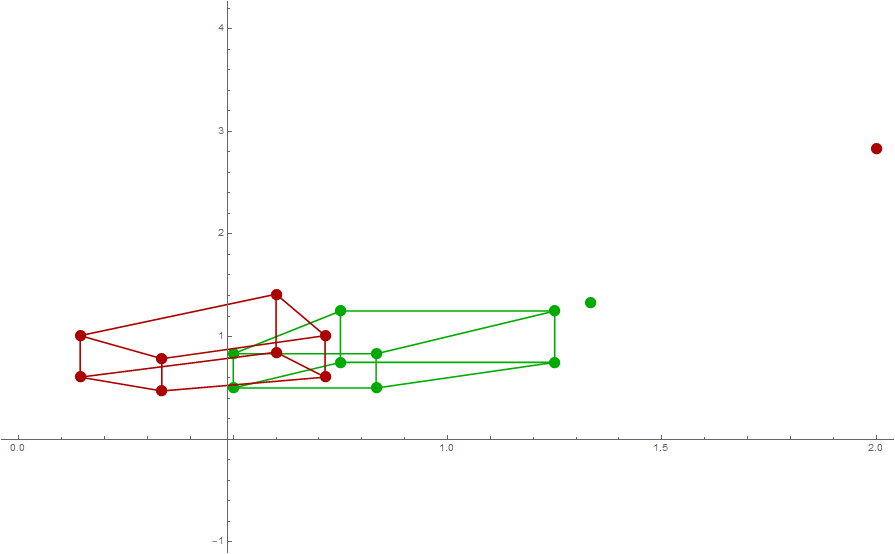
\includegraphics[width=\linewidth]{images/Zeta1.png}
	\caption[Abbildungen bei $K' = K$]{$C$ und $C'$ haben die selbe Auflösung eingestellt}
	\label{fig:K}
	\endminipage\hfill
	\minipage{0.48\textwidth}
	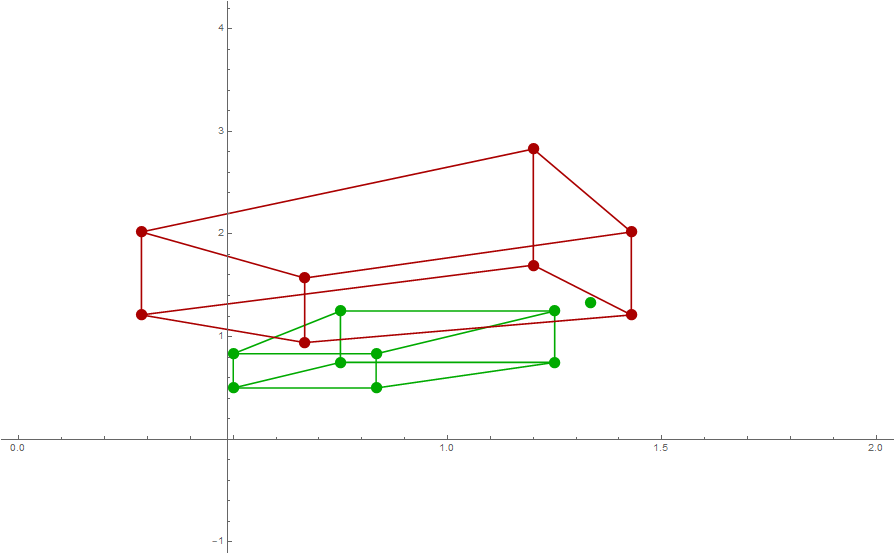
\includegraphics[width=\linewidth]{images/Zeta2.png}
	\caption[Abbildung bei $K'_1$]{$C$ und $C'$ haben unterschiedliche Auflösungen eingestellt. $C$ mit $K$ und $C'$ mit $K_1'$}
	\label{fig:K1}
	\endminipage\hfill
\end{figure}

\begin{figure}[!htb]
	\minipage{0.48\textwidth}
	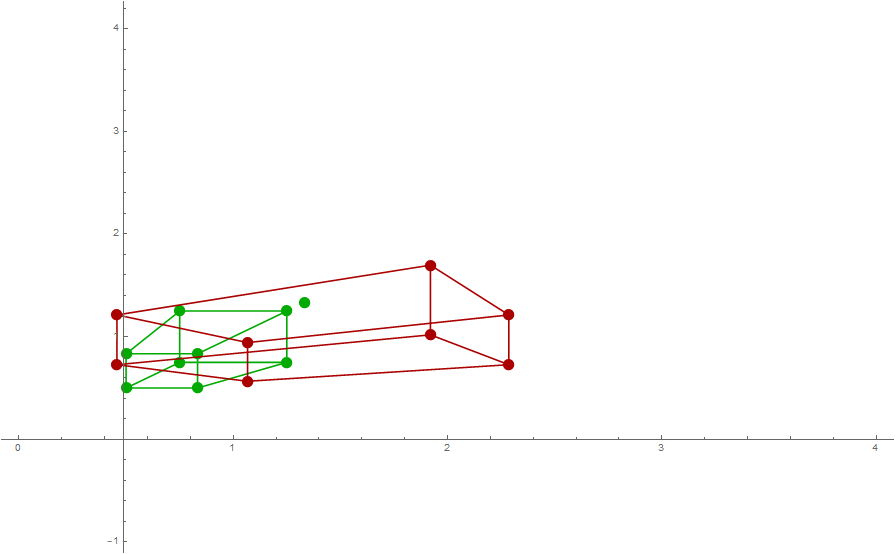
\includegraphics[width=\linewidth]{images/Zeta32_12.png}
	\caption[Abbildungen bei $K'_2$]{$C$ mit $K$ und $C'$ mit $K_2'$}
	\label{fig:K2}
	\endminipage\hfill
	\minipage{0.48\textwidth}
	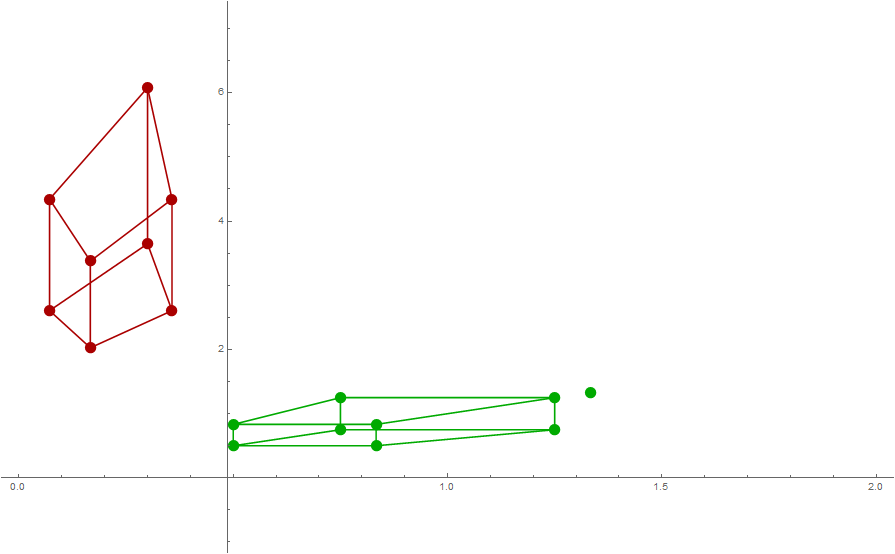
\includegraphics[width=\linewidth]{images/Zeta05_43.png}
	\caption[Abbildungen bei $K'_3$]{$C$ mit $K$ und $C'$ mit $K_3'$}
	\label{fig:K3}
	\endminipage\hfill
\end{figure}
\pagebreak

Wird das synthetische Beispiel jeweils mit den drei verschiedenen modifizierten $K'$ durchgerechnet, so ergeben sich für die essentielle Matrix folgende Ergebnisse.\\

\begin{gather*}
	\zeta'_x = 1, \, \zeta'_y = 1: \; \; \;\;
	E = \begin{pmatrix}
		0&-0.5&0\\
		0&0&\frac{1}{\sqrt{2}}\\
		0&0.5&0
	\end{pmatrix} |: 0.5 \; \leadsto
	E = \begin{pmatrix}
		0&-1&0\\
		0&0&-\sqrt{2}\\
		0&1&0
	\end{pmatrix}\\
	\zeta'_x = 2, \, \zeta'_y = 2: \; \; \;\;
	E = \begin{pmatrix}
		0&0.756&0\\
		0&0&1.069\\
		0&-0.756&0
	\end{pmatrix} |: -0.756 \; \leadsto
	E = \begin{pmatrix}
		0&-1&0\\
		0&0&-\sqrt{2}\\
		0&1&0
	\end{pmatrix}\\
	\zeta'_x = 3.2, \, \zeta'_y = 1.2: \; \; \;\;
	E = \begin{pmatrix}
		0&0.634&0\\
		0&0&1.069\\
		0&-0.634&0
	\end{pmatrix} |: -0.634 \; \leadsto
	E = \begin{pmatrix}
		0&-1&0\\
		0&0&-\sqrt{2}\\
		0&1&0
	\end{pmatrix}\\
	\zeta'_x = 0.5, \, \zeta'_y = 4.3: \; \; \;\;
	E = \begin{pmatrix}
		0&0.442&0\\
		0&0&1.069\\
		0&-0.442&0
	\end{pmatrix} |: -0.442 \; \leadsto
	E = \begin{pmatrix}
		0&-1&0\\
		0&0&-\sqrt{2}\\
		0&1&0
	\end{pmatrix}\\
\end{gather*}

Wie beobachtet werden kann, werden, trotz unterschiedlicher Kameraauflösungen für $K'$, immer die selbe essentielle Matrix im Algorithmus bestimmt. Zu Erinnerung, in Kapitel \ref{sec:HFE} wurde gezeigt, dass jedes Vielfache von $E$ ist eine gültige Lösung ist. Somit gilt die Behauptung, dass die Kameraauflösung keine Auswirkung auf die Bestimmung der extrinsischen Kameraparameter hat, im synthetischen Beispiel, als bestätigt. Als Vergleich kann die Abbildung \ref{fig: reconstructedDifferentResolutions}, welche das Ergebnis der Rekonstruktion der Szene mit $K'_3$ als Kameramatrix für $C'$ veranschaulicht, mit der Rekonstruierten Szene in Abbildung 	\ref{fig:Quader1} aus dem ersten Beispiel, betrachtet werden. Für die anderen Varianten von $K'$ wurden ebenfals die selbe 3D-Szene rekonstruiert.\\ 





\begin{figure}[!htb]
	\centering
	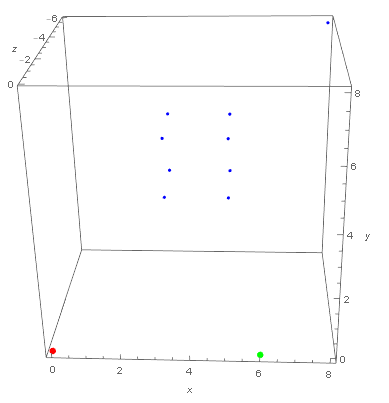
\includegraphics[width=0.5\linewidth]{images/DifferentAufloesungRekonstructedScene.png}
	\caption[Rekonstruierte Szene bei unterschiedlichen Kameraauflösungen]{Die Abbildung zeigt die rekonstruierte Szenen des synthetischen Beispiels mit $K'_3$ als intrisische Parameter für $C'$.} 
	\label{fig: reconstructedDifferentResolutions}
\end{figure}



